\documentclass[a4paper,12pt]{article}

\title{Exercise 5: Self Localization}
\author{Group 6:\\Niels\\Troels\\Mark\\Kristian}

\usepackage[T1]{fontenc}
\usepackage{lmodern}
\usepackage[utf8]{inputenc}
\usepackage[british]{babel}
\usepackage{microtype}
\usepackage{underscore}
\usepackage{amsmath}
\usepackage{graphicx}
\usepackage[hidelinks]{hyperref}

\setlength{\parskip}{1ex}
\setlength{\parindent}{0pt}
\setlength{\parfillskip}{30pt plus 1 fil}

\begin{document}

\maketitle
\newpage
\section{Implementation}

To build the code, run \texttt{make}.  It builds the program
\texttt{exercise5}.  We use OpenCV 2.4.


\section{Particle Filter}

\begin{figure}[!h]
\centering
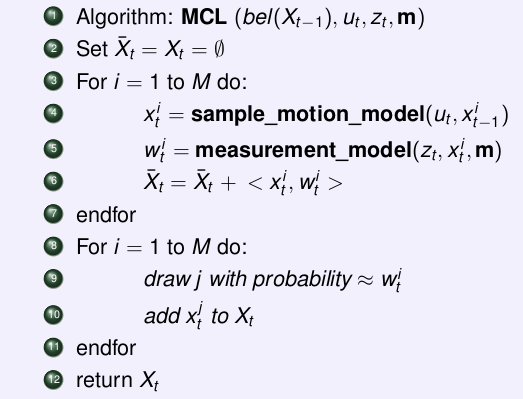
\includegraphics[scale=0.50]{MCL.png}
\caption{MCL localization algorithm}
\label{MCL}
\end{figure}

\subsection{Prediction step}

For the prediction step we use the function move_particle in particle.cc. It
corresponds with the sample_motion_model as in algorithm.

The move_particle is fairly simple, It simply moves the particle position(x,y)
with the given $\Delta x $ and $\Delta y$ if the control command were drive. If
the robot turned we add $\Delta \theta$ to the particle $\theta$ value.

The given delta values are calculated with the robot speed and driving time. 

\begin{align*}
\Delta x &= \cos(p.\theta)\cdot\text{speed}\cdot 100\\
\Delta y &= \sin(p.\theta)\cdot\text{speed}\cdot 100
\end{align*}

After every prediction step we add some noise to the prediction with the
function add_uncertainty with parameters 5 cm and 5 degrees.

\subsection{Calculating weights}

The weight of the particle can be calculated using hint 6 in the exercise. Thus
the weight of the particle is the product: $p(d_M | x^{(i}, y^{(i)})) \cdot
p(\theta_M |x^{(i)} , y^{(i)} , \theta^{(i)} ) $.

The weights of the particle is calculated at landmark detection. The given code
returns the distance and orientation to the landmark which we use the product.

The product consist of the gauss-distribution, so our implementation takes a
difference and variance argument. The difference is either the difference
between particle and landmark in dist or angle orientation.

After we calculated all the weights we normalize the particle weights by
dividing with the total sum of weights.

\subsection{Resampling}

In order to resample we create a sum vector with consists of the cumulative sum
of every particle weight which we use when we pick random an particle. By
creating a cumulative sum vector we remove the possibility of particles with a
weight of zero is getting picked.

When we pick particles we generate a random number z with randf().

Then we run through the sum vector until we get an entry which equal of greater
than z. When this occurs we pick that particle with the given index. This is
done num_particles times, so we have consistent number of particles.

Each time we pick a particle we add it to a new vector which is set to be our
working set of particles at the end of resampling.

This does unfortunately not work in practice of reasons we do not know. so
created a more naive implementation:

\begin{enumerate}
\item All particles are in the array \texttt{particles}.
\item Create an empty array \texttt{particles_resampled}.
\item While the size of \texttt{particles_resampled} is less than the size of
\texttt{particles}, do:
\begin{enumerate}
\item Pick a random index \texttt{i} in \texttt{particles}.
\item If the weight of \texttt{particles[i]} is above a random number between
$0$ and $1$, append \texttt{particles[i]} to \texttt{particles_resampled}.
\end{enumerate}
\end{enumerate}

This should still satisfy the requirement that a particle is picked with the
probability of its weight, but it is not very efficient (and in theory it might
not terminate).


\section{Driving Strategy}

We use a state-based approach for our driving strategy: We split the strategy
into multiple states, and let each state handle a small part.  The driving
strategy code is part of the main loop.

\begin{description}
\item[searching]\hfill\\
This is the start state.  The robot turns counter-clockwise until it recognizes
a landmark, after which it goes to state \textbf{align}.

\item[align]\hfill\\
The robot aligns itself to point directly at the recognized landmark (within
a low threshold).  Once aligned, it goes to state \textbf{approach}.

\item[approach]\hfill\\
We don't want the robot to be too far away from the landmark.  If the robot is
more than 150 cm from the landmark, the robot approaches it.  Once it's at most
150 cm away, it goes to state \textbf{drive_around_landmark}.

If the robot is not directly in front of the landmark, it goes back to the state
\textbf{align}.

\item[drive_around_landmark]\hfill\\
At this point the robot has seen the first landmark, and we now want it to find
the second landmark.  The robot drives around the first landmark in a square and
keeps checking for the second landmark.  This should explore all angles.  Once
it finds the second landmark, it goes to state \textbf{triangulating}.

\item[triangulating]\hfill\\
We run the particle filter a few times.  The robot then goes to state
\textbf{drive_to_center}.

\item[drive_to_center]\hfill\\
The robot has now seen both landmarks, and we choose to trust its estimated
coordinates.  The robot drives towards $(150, 0)$ and then goes to state
\textbf{arrived_at_center}.

\item[arrived_at_center]\hfill\\
Success!
\end{description}


\section{Discussion}

We have tested the code quite a bit, both in Stage with webcam, and on a
Scorpion robot.

\subsection{Particle Filter}

We have tested the particle filter independently of the driving, and it looks
okay.  For example, see figure~\ref{fig:particle-test} for the case where the
first landmark has been detected, and the particle filter has resampled the
particles to form a circle around the landmark.

\begin{figure}[!h]
\centering
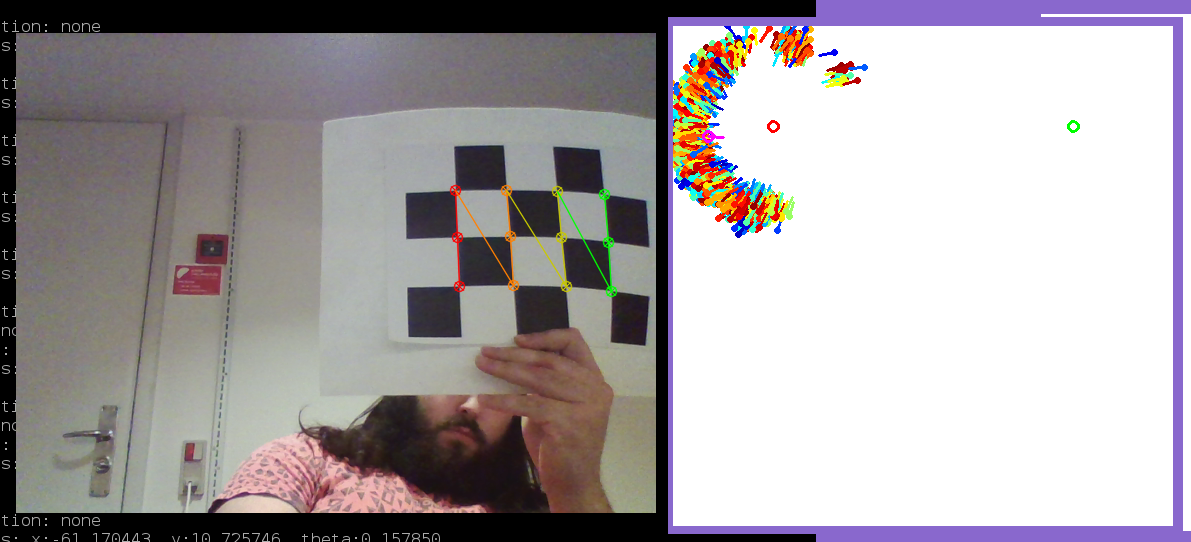
\includegraphics[width=.9\textwidth]{partikeltest.png}
\caption{Test of the particle filter.  The code recognizes the horizontal
landmark and shows the particles.}
\label{fig:particle-test}
\end{figure}


\subsection{Actual Driving}

While the particle filter appears to work okay, we have not managed to fully
integrate it with the driving strategy.  The Scorpion has occasionally driven
close to the center, but sometimes it drives far off.  We have several ideas for
why this might be:

\begin{description}
\item[Wrong camera calibration]\hfill\\
The estimated distance to the landmark is sometimes off by up to 30 cm on an
actual distance of just over a meter.  This might be due to a bad camera
calibration, so maybe we should recalibrate.

\item[Weird turning angles]\hfill\\
Sometimes the robot turns at a planned junction, but apparently in the wrong
direction.  This is probably a bug in one of the states.
\end{description}


\end{document}
